\begingroup
\setlength{\tabcolsep}{0pt}
\renewcommand{\arraystretch}{0.55} % Default value: 1
\setlength{\fboxsep}{1mm}
\begin{table*}
\centering
\begin{tabular}{|P{2cm}|P{1.3cm}|P{2cm}|P{1.5cm} A P{1.5cm}|P{8cm}|}
\hline
Technique & Interval & Reduction & Data & Avg$_{L2}$ & Cell  & \multirow{2}{*}{Scatter Plot} \\
& & & (GB) & & Side\% & \\
\cline{1-6}
\multirow{3}{*}{\textcolor{blue!80}{\textbf{Eulerian}}} & 20 & \multirow{3}{*}{Full Res} & 267 & 0.0197 & 116.1 & \multirow{12}{*}{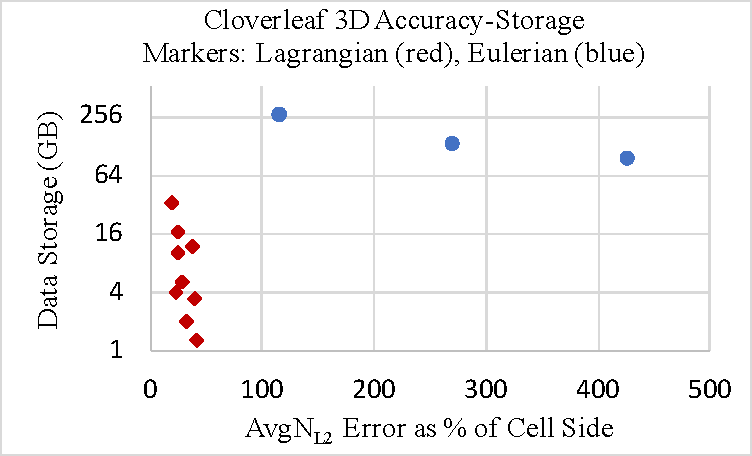
\includegraphics[width=0.95\linewidth]{images/cloverleaf_accuracy.pdf}} \\
\cline{2-2}\cline{4-6}
& 40 & & 133 & 0.0459 & 270.4 & \\
\cline{2-2}\cline{4-6}
%\hline
& 60 & & 95 & 0.0725 & 426.9 &  \\
\cline{1-6}
\multirow{9}{*}{\textcolor{BrickRed}{\textbf{Lagrangian}}} & \multirow{3}{*}{20} & 1:8 & 34 & 0.0032 & 18.9 & \\
\cline{3-3}\cline{4-6}
%\hline
 & & 1:27 & 10 & 0.0040 & 23.8 & \\
\cline{3-3}\cline{4-6}
%\hline
 & & 1:64 & 4 & 0.0040 & 23.5 & \\
\cline{2-6}
& \multirow{3}{*}{40} & 1:8 & 17 & 0.0043 & 25.6 &  \\
\cline{3-3}\cline{4-6}
%\hline
& & 1:27 & 5.1 & 0.0049 & 29.1 &  \\
\cline{3-3}\cline{4-6}
%\hline
& & 1:64 & 2 & 0.0053 & 31.3 & \\
\cline{2-6}
& \multirow{3}{*}{60} & 1:8 & 12 & 0.0064 & 37.8 & \\
\cline{3-3}\cline{4-6}
%\hline
& & 1:27 & 3.4 & 0.0066 & 39 & \\
\cline{3-3}\cline{4-6}
%\hline
& & 1:64 & 1.3 & 0.0070 & 41.2 & \\
\hline
\end{tabular}
\vspace{2mm}
\caption{Cloverleaf 3D Accuracy-Data Storage Results. 
%
For this experiment, we ran a $586^3$ simulation grid using 96 MPI ranks (1 GPU each) across 16 compute nodes for 600 cycles.
%
In this table, we report total data storage costs and accuracy measurements. 
%
The Configuration column contains information regarding \textbf{interval}, i.e., number of cycles between storing data to disk, and \textbf{number of particles}, i.e., the data reduction. 
%
Columns Average L2-norm and End Point present the average results for 100,000 test particles. 
%
The \% Cell side column presents the average L2-norm value as a percentage of the simulation grid cell side (0\% would indicate no error; 100\% indicates error size is equal to the simulation grid cell side).}
\end{table*}
\endgroup
